\section{Updates}
\begin{frame}
    \frametitle{My previous plots overbroadened BWs2+C}
    \begin{figure}
        \centering
        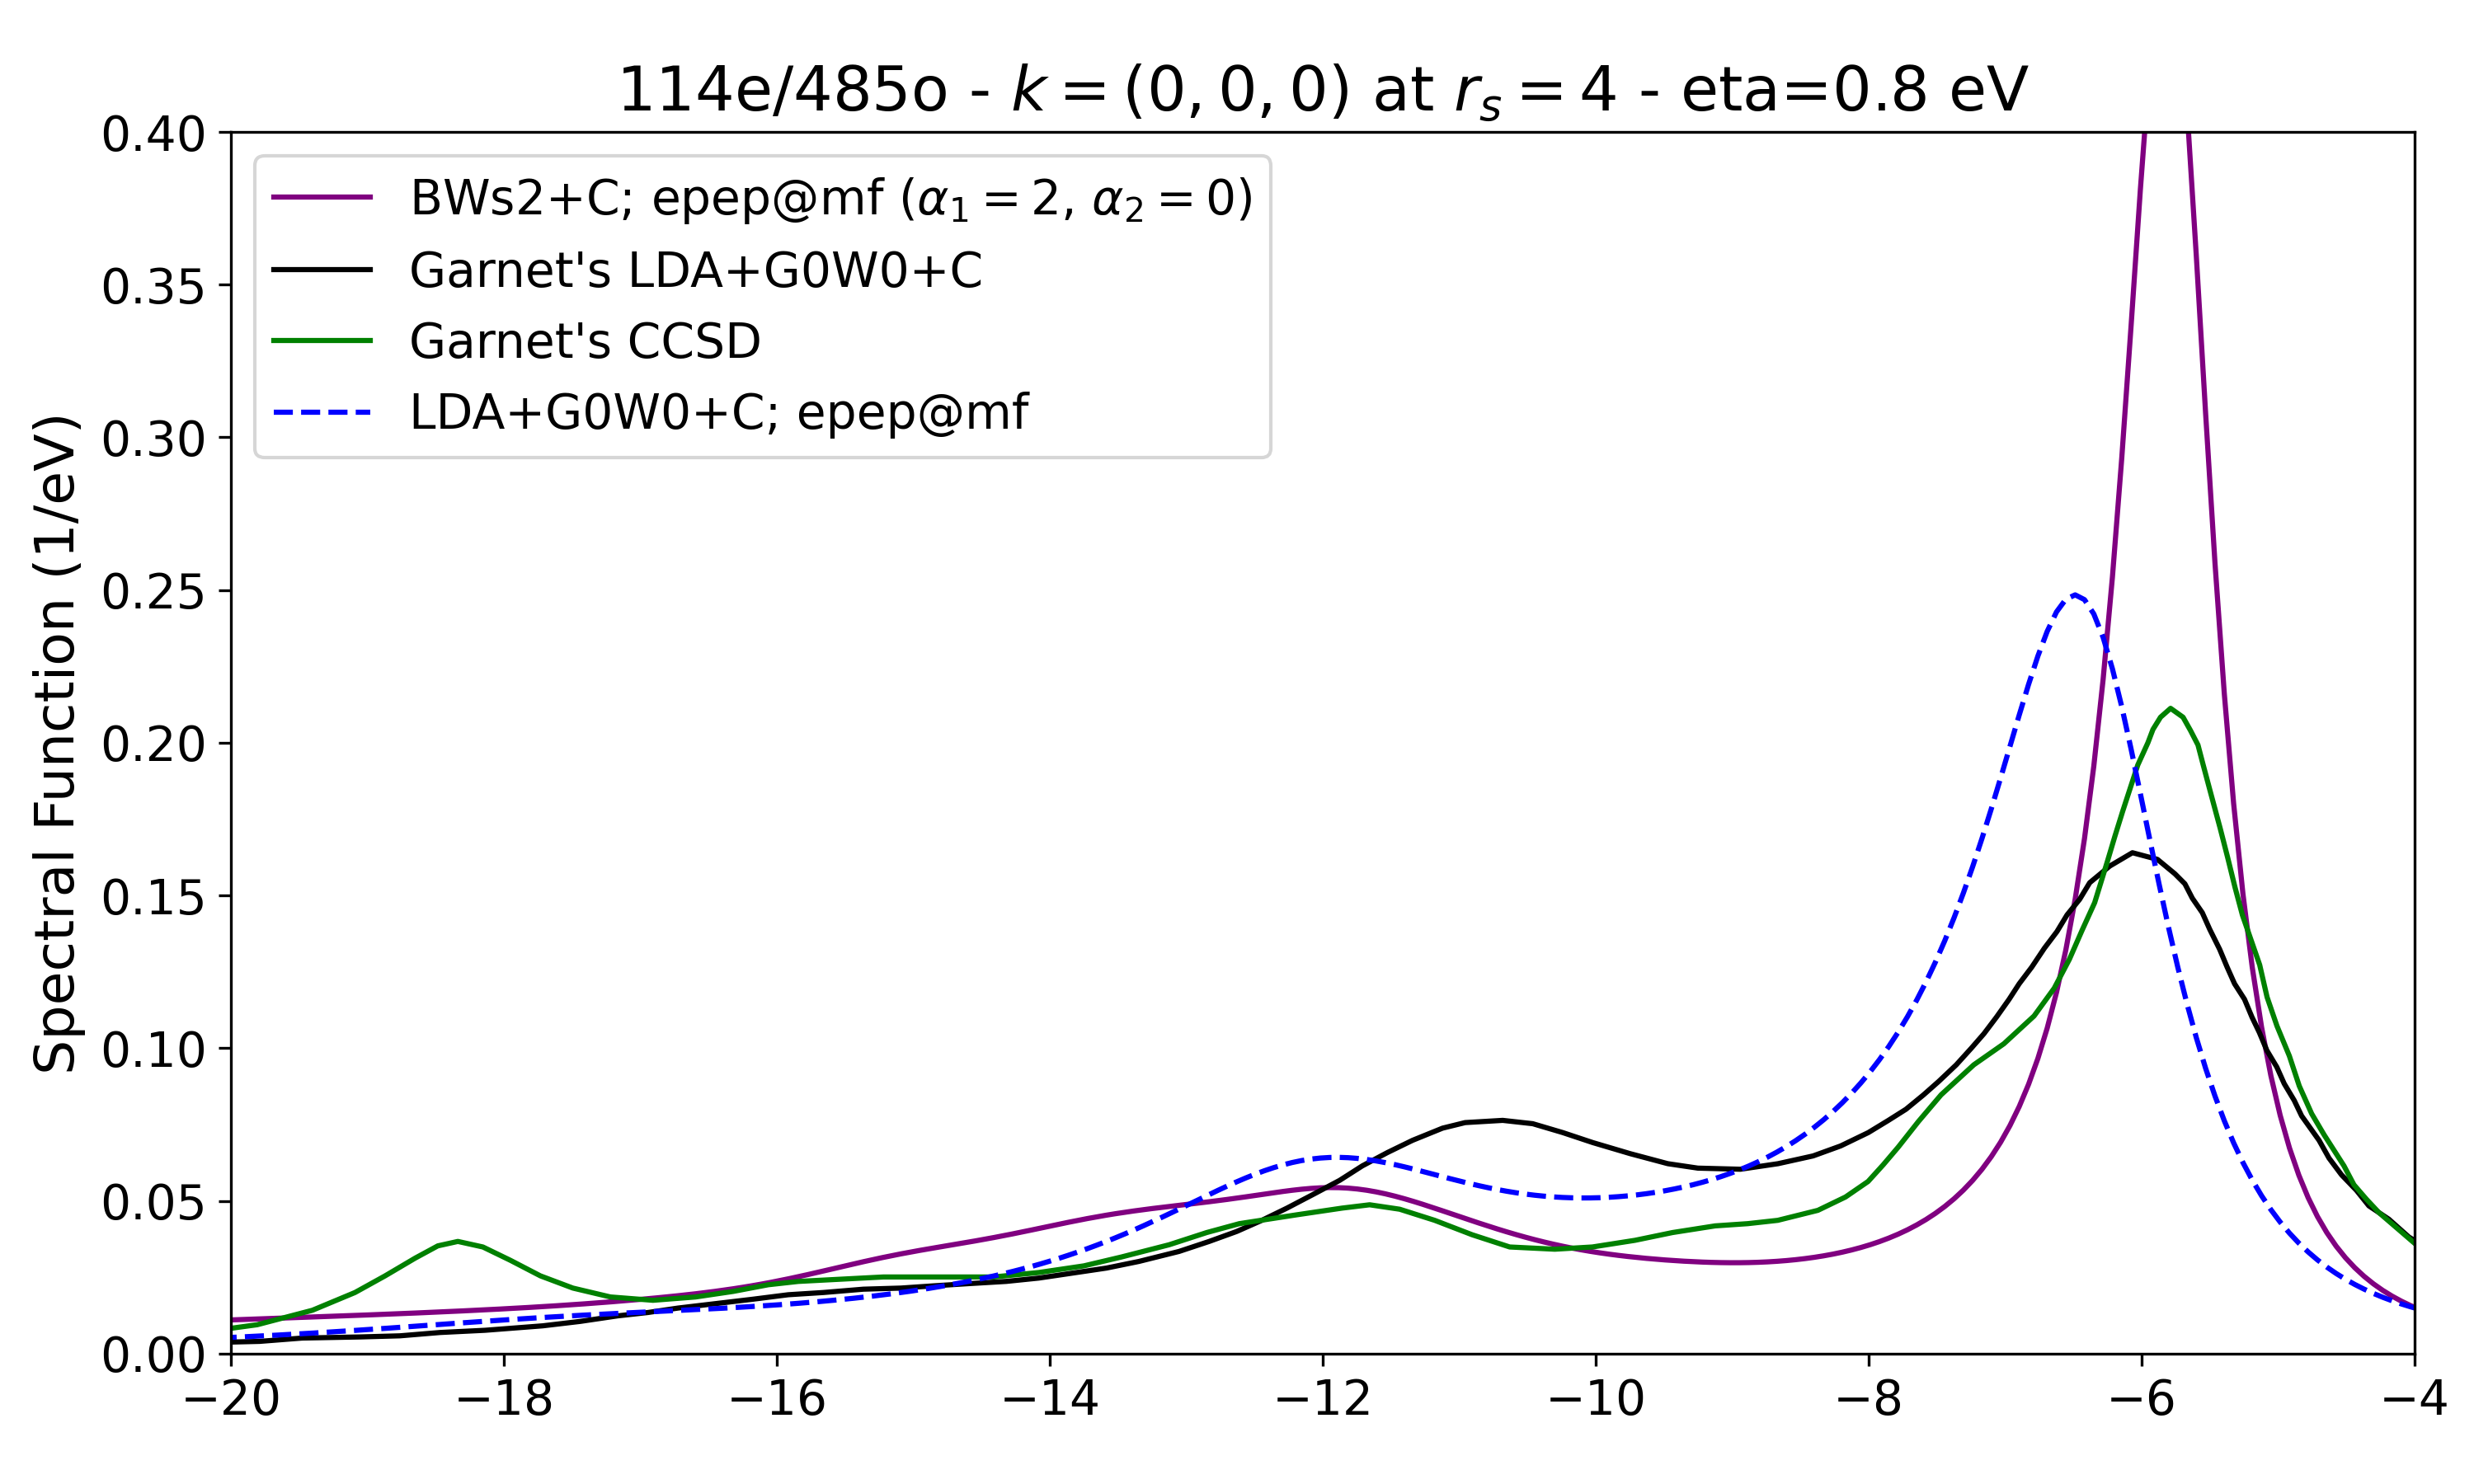
\includegraphics[width=\textwidth]{26/7/7-31/refpgw.png}
        % \caption{LDA+GW}
    \end{figure}
\end{frame}
\begin{frame}
    \frametitle{TDL comparison with references}
    \begin{figure}
        \centering
        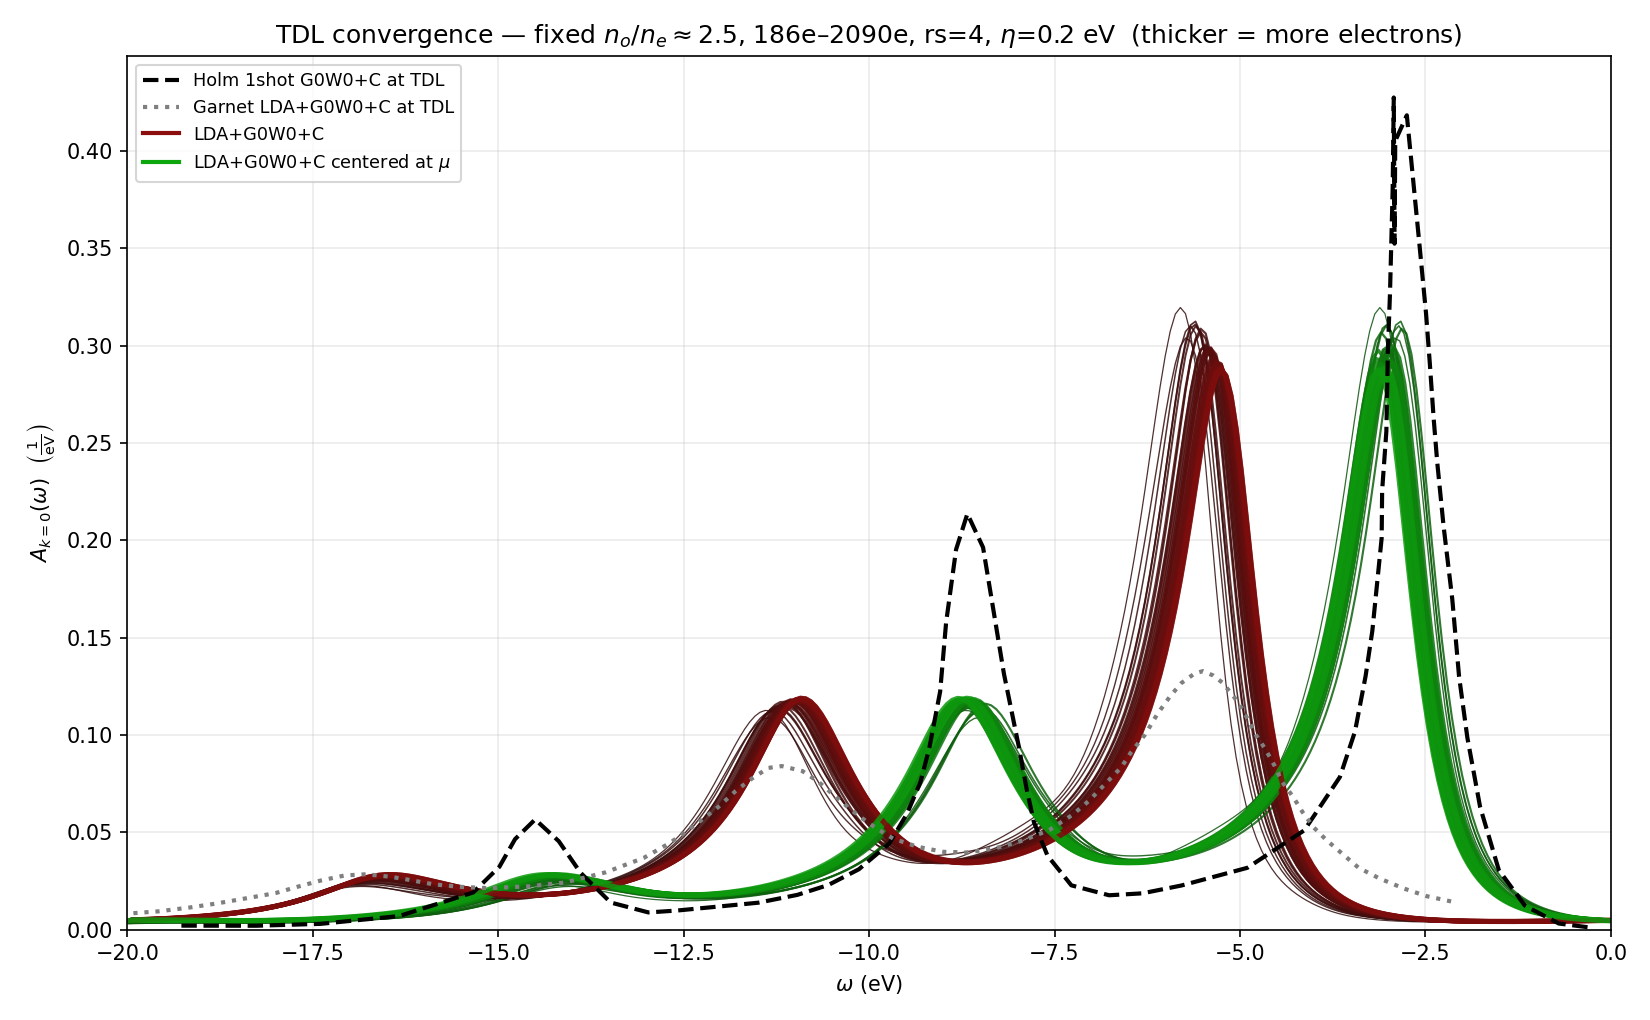
\includegraphics[width=\textwidth]{26/7/7-31/tdl_stream_overlay.png}
        % \caption{LDA+GW}
    \end{figure}
\end{frame}
\begin{frame}
    \frametitle{TDL convergence}
    \begin{figure}
        \centering
        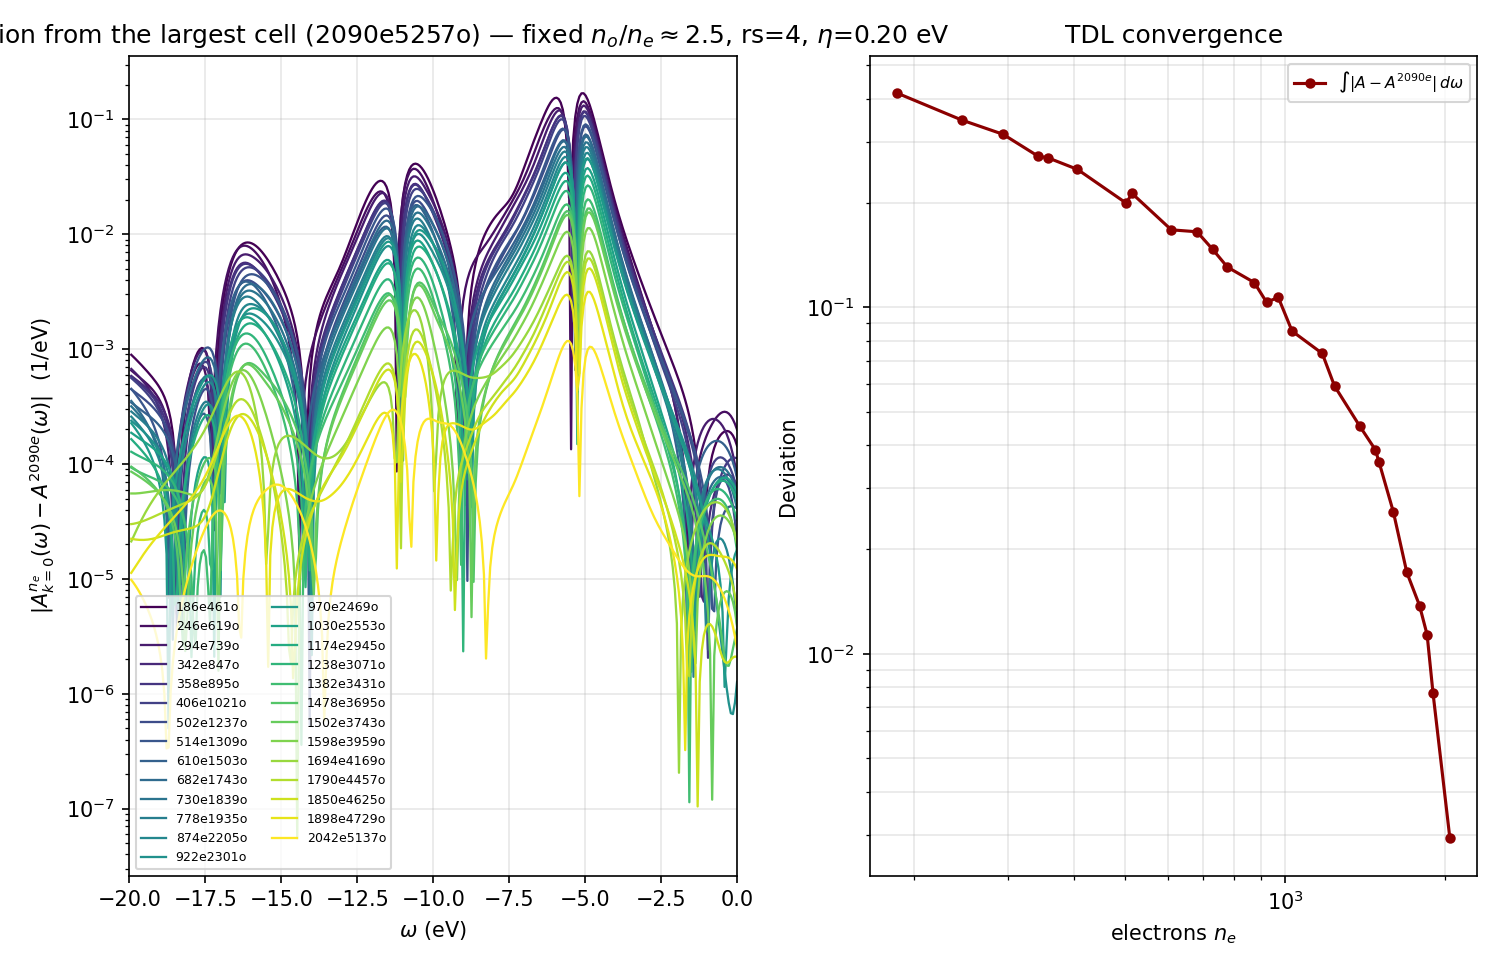
\includegraphics[width=\textwidth]{26/7/7-31/tdl_stream_diff.png}
        % \caption{LDA+GW}
    \end{figure}
\end{frame}

\section{SCCE(GW0) in a finite basis}
\begin{frame}
    \frametitle{Holms' paper}
    \begin{itemize}
        \item Fitting to Gaussians isn't practical for finite broadening \pause
        \item Landau form remains central
    \end{itemize}
\end{frame}
\begin{frame}
    \frametitle{Insights from reorganizing the Landau form}
\begin{align}
    C_{k}^R(t) &= \int d\omega \frac{\beta_{k}(\omega)}{\omega^2} \left( e^{-i\omega t} + i\omega t - 1 \right) \\
&= \underbrace{\int d\omega \frac{\beta_{k}(\omega)}{\omega^2} \left( e^{-i\omega t} - 1 \right)}_{C_k^{sat}(t)} + i t \underbrace{\int d\omega \frac{\beta_{k}(\omega)}{\omega}}_{\Delta_k} \\
&= C_k^{sat}(t) + i \Delta_k t
\end{align}
\pause
Since $\Delta_k=-\operatorname{Re}\Sigma^c_k(E_k^{GW})$, we can write
\begin{align}
    G^{R}_{k}(t)
    &= -i \Theta(t) e^{-i(\epsilon_k + \operatorname{Re} \Sigma_{c, k}^R(E)) t} e^{C_k^{sat}(t)} \\
    &= -i \Theta(t) e^{-i(E_k^{QP}) t} e^{C_k^{sat}(t)}.
\end{align}

\end{frame}
\begin{frame}
    \frametitle{Self-consistent scheme}
After the initial iteration, self-energy updates become 
\begin{equation}
    \Sigma_{k, c}^R(t)=\theta(t)\left[-\sum_{m<k_F, I}\left|M_{ k, m}^I\right|^2 G_{m,CE}^{<}(t) e^{+i \Omega_I t} + \sum_{m>k_F, I}\left|M_{ k, m}^I\right|^2 G_{m,CE}^{>}(t) e^{-i \Omega_I t}\right]
\end{equation}
and then DFT to get $\Sigma_{k, c}^R(\omega)$. \pause We can try three schemes
\begin{enumerate}
    \item update $E_k^{QP} = \epsilon_k + \operatorname{Re} \Sigma_{c, k}^R(E_k^{QP})$, but keep $C_k^{sat}(t)$ fixed \pause
    \item update $\beta_k^{\text{sat}}(\omega)$ and thus also $C_k^{sat}(t)$, but keep $E_k^{QP}$ fixed \pause
    \item update both $E_k^{QP}$ and $C_k^{sat}(t)$ 
\end{enumerate}
\end{frame}
\section{Connection to CCGF}
\begin{frame}
    \frametitle{Ground State of the Electronic Polaron in the IBM}
Hamiltonian is 
\begin{equation}
H_{\rm ch}
=
E_{\rm ch}
+
\sum_\nu
\Omega_\nu Q_\nu^\dagger Q_\nu
+
\sum_\nu
\left(
M_\nu Q_\nu^\dagger
+
M_\nu^* Q_\nu
\right).
\end{equation}
\pause
The ground state of the electronic Poluron is a coherent state of QB operators $Q_\nu$ as
\begin{equation}
    |\Theta_{ch}\rangle = D(\beta)\left|0_{\mathrm{RPA}}\right\rangle.
\end{equation} 
\pause
The displacement operator is defined as
\begin{equation}
    D(\beta)=\exp \left[\sum_\mu\left(\beta_\mu Q_\mu^{\dagger}-\beta_\mu^* Q_\mu\right)\right] .
\end{equation}
where $\beta_\mu = -M_\mu / \Omega_\mu$.
\end{frame}
\begin{frame}
    \frametitle{Green's function of the electronic polaron}
Using the shifted QB operators
\begin{equation}
\widetilde Q_\nu
=
Q_\nu
- \beta_\nu
\qquad
\widetilde Q_\nu^\dagger
=
Q_\nu^\dagger
+
\beta_\nu^*,
\end{equation}
of which $\left|0_{\mathrm{RPA}}\right\rangle$ is a coherent state,
\pause we can rewrite the Hamiltonian as
\begin{equation}
H_{\rm ch}
=
E_{\rm pol}
+
\sum_\nu
\Omega_\nu
\widetilde Q_\nu^\dagger \widetilde Q_\nu ,
\end{equation}
where $E_{\rm pol}=E_{\rm ch}-\sum_\nu \Omega_\nu |\beta_\nu|^2$. \pause Then
\begin{align}
G^{QB,R}_{\rm ch}(t)
&=
-i \theta(t)
\left\langle 0_{\rm RPA} \right|
e^{-i H_{\rm ch} t}
\left|0_{\rm RPA}\right\rangle
\\
% &=-i \theta(t) e^{-i E_{\mathrm{pol}} t}\left\langle 0_{\mathrm{RPA}}\right| e^{-i \sum_\nu \Omega_\nu \tilde{Q}_\nu \tilde{Q}_\nu t}\left|0_{\mathrm{RPA}}\right\rangle \label{eq:G_ch_t} \\
% &=
% -i \theta(t)
% e^{-i E_{\rm pol} t}
% \exp
% \left[
% \sum_{\nu}
% |\beta_{\nu}|^2
% \left(
% e^{-i \Omega_{\nu} t}
% -
% 1
% \right)
% \right]
% \\
&=
-i \theta(t)
e^{-i E_{\rm pol} t}
\underbrace{
\exp
\left[
-\sum_{\nu} |\beta_{\nu}|^2
\right]
}_{Z_{\rm pol}}
\prod_{\nu}
\exp
\left[
|\beta_{\nu}|^2 e^{-i\Omega_{\nu} t}
\right]
\\
% &=
% -i \theta(t)
% Z_{\rm pol}
% e^{-i E_{\rm pol} t}
% \prod_{\nu}
% \sum_{n_{\nu}=0}^{\infty}
% \frac{
% |\beta_{\nu}|^{2n_{\nu}}
% }{
% n_{\nu}!
% }
% e^{-i n_{\nu} \Omega_{\nu} t}
% \\
&=
-i \theta(t)
Z_{\rm pol}
\sum_{\mathbf n}
\left[
\prod_{\nu}
\frac{
|\beta_{\nu}|^{2n_{\nu}}
}{
n_{\nu}!
}
\right]
\exp
\left[
-i
\left(
E_{\rm pol}
+
\sum_{\nu} n_{\nu}\Omega_{\nu}
\right)t
\right].
\end{align}
\end{frame}
\begin{frame}
    \frametitle{Connection between the cumulant and the CCGF in this formalism}
If instead of the IBM, we consider
\begin{equation}
H_p^{\rm eff}
=
\epsilon_p^{\rm HF}
+
\sum_{m\nu}
\Delta_{pm\nu}
B_{pm\nu}^{\dagger}
B_{pm\nu}
+
\sum_{m\nu}
\left(
\mathcal{M}_{pm\nu}
B_{pm\nu}^{\dagger}
+
\mathcal{M}_{pm\nu}^{*}
B_{pm\nu}
\right),
\end{equation}

then we recover the G0W0+C Green's function. \pause We can make contact with the CCGF, by instead considering the Hamiltonian
\begin{equation}
H_{\mathrm{ch}}=E_{\mathrm{ref}}^{\mathrm{ch}}+\sum_{p q} f_{p q}^{\mathrm{ch}}\left\{a_p^{\dagger} a_q\right\}+\frac{1}{4} \sum_{p q r s} v_{p q r s}^{\mathrm{ch}}\left\{a_p^{\dagger} a_q^{\dagger} a_s a_r\right\},
\end{equation}
which leads to the CCGF.
\end{frame}
